\documentclass[11pt]{article}
\usepackage{../EllioStyle}
\usepackage{listings}
\usepackage{mathtools}

\definecolor{codegreen}{rgb}{0,0.6,0}
\definecolor{codegray}{rgb}{0.5,0.5,0.5}
\definecolor{codepurple}{rgb}{0.58,0,0.82}
\definecolor{backcolour}{rgb}{0.95,0.95,0.92}

\graphicspath{ {imgs/} }

\title{Project}
\author{Elliott Pryor}
\date{5 December 2023}

\rhead{Project}
\lhead{Elliott Pryor}

\begin{document}
\maketitle

\problem{1}
Consider the system
$$
G(s) = \frac{50(s+3)}{s(s+2)(s+5)}
$$

\begin{enumerate}[a)]
    \item Use Bode plot to design a lead compensator $C(s)$ with unity DC gain so that the phase marginS of the closed-loop system is no less than 40\degree.
    \item Use MATLAB to verify the resulting phase marginally
    \item What is the bandwidth of the resulting closed-loop system?
\end{enumerate}

\begin{figure}[h] 
    \centering
    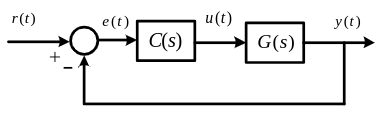
\includegraphics[width=0.55 \linewidth]{12-04-p1.png}
    \caption{Problem1}
    \label{fig:p1}
\end{figure}

\soln







\problem{2}
Consider the system
$$
G(s) = \frac{K}{s(s/5 + 1)(s/250 + 1)}
$$
\begin{enumerate}[a)]
    \item Use Bode to design a lag compensator $C(s)$ so that the closed loop system satisfies:
    \begin{itemize}
        \item The steady state error to a unit ramp reference input is less than 0.01
        \item The phase margin is no less than 40\degree
    \end{itemize}
    \item Use MATLAB to verify the resulting phase margin
\end{enumerate}
\begin{figure}[h] 
    \centering
    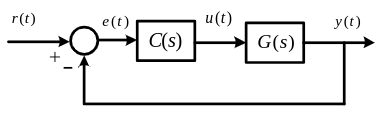
\includegraphics[width=0.55 \linewidth]{12-04-p1.png}
    \caption{Problem2}
    \label{fig:p2}
\end{figure}

\soln











\problem{3}
Given the state space model of a system:

\begin{align*}
    \dot{x} &= \begin{bmatrix}
        2 & 1 \\ -1 & 1
    \end{bmatrix} x + \begin{pmatrix}
        1 \\ 2
    \end{pmatrix} u \\
    y &= \begin{pmatrix}
        1 & 1
    \end{pmatrix} x
\end{align*}

\begin{enumerate}[a)]
    \item Find the state feedback gain $F$ such that the closed-loop system has -1 and -2 at its poles.
    Compute $F$ without using any state transformation.
    \item Design an observer to estimate the state of the system. Select the poles for the error dynamics to be $-2 \pm 2i$
    \item Construct an observer-based output feedback law that stabilizes the system.
\end{enumerate}
\soln








\problem{4}
Complete the class evaluation:
\soln

Yes

\end{document}